%%%%%%%%%%%%%%%%%%%%%%%%%%%%%%%%%%%%%%%%%%%%%%%%
% 
% == CSIM Handout LaTeX Template ==
% == Credit ==
% Assoc. Prof. Matthew N. Dailey 
% Computer Science and Information Management 
% Asian Insitute of Technology 
% 
%%%%%%%%%%%%%%%%%%%%%%%%%%%%%%%%%%%%%%%%%%%%%%%%

\documentclass{article}

\usepackage{a4,url,upquote}
\usepackage{graphicx}
\usepackage{hyperref}
\usepackage[cmex10]{amsmath}
\usepackage{amssymb}

\setlength{\textwidth}{6.5in}
\setlength{\textheight}{9in}
\setlength{\oddsidemargin}{0in}
\setlength{\evensidemargin}{0in}
\setlength{\topmargin}{0in}
\setlength{\headheight}{0in}
\setlength{\headsep}{0in}
\setlength{\footskip}{0.5in}

\newcommand{\bheading}[1]{\vspace{10pt} \noindent \textbf{#1}}

\begin{document}

\begin{tabbing}
  \`\=\kill
%  \input{2011-Header}
  \textbf{Workshop:} Machine Learning in Computer Vision
  \` April 8, 2013 \\ 
  Asian Institute of Technology 
  \` Computer Science and Information Management \\ 
  \textbf{Handout:} Shadow Detection
  \` \textbf{Instructor:} Matthew N.\ Dailey (\tt{\small mdailey@ait.asia})
\end{tabbing}

\hrule

\vspace{.25in}

\begin{center}
\textbf{\Large Shadow Detection}
\end{center}

\vspace{.15in}

\noindent \textbf{Instructions:} In this tutorial, you will learn how
to use the simple approaches for detecting shadows. \\

\noindent \textbf{Prerequisites:} You need to have OpenCV and
Matlab/Octave installed on your machine.

\begin{itemize}
  \item OpenCV Install Guide --
    \url{http://opencv.willowgarage.com/wiki/InstallGuide}
  \item Octave Install Guide --
    \url{http://wiki.octave.org/Main_Page#Installation_Instructions_for_Windows.2C_MacOS_X_and_GNU.2FLinux}
\end{itemize}

% Inserting a tilde into LaTeX
% Credit:
% http://tex.stackexchange.com/questions/9363/how-does-one-insert-a-backslash-or-a-tilde-into-latex

\subsection*{Folders and Files Included in this Tutorial}

\begin{itemize}
  \item[-] {\tt code} - Folder that contains code and scripts
  \begin{itemize}
    \item[-] {\tt shadow\_utils.h} and {\tt shadow\_utils.cc} -- C/C++
      code that defines and implements data structures and functions
      needed to used.
    \item[-] {\tt shadow\_hsv.cc} -- C/C++ code that implements the
      HSV-based thresholding method.
    \item[-] {\tt shadow\_ncc.cc} -- C/C++ code that implements the
      normalized cross-correlation method.
    \item[-] {\tt shadow\_ml.cc} -- C/C++ code that implements the
      maximum likelihood method.
    \item[-] {\tt get\_data\_under\_mask.cc} -- C/C++ code that is used
      for extracting the difference in hue, saturation, and value
      componets between the current frame and the background.
    \item[-] {\tt extract\_color\_information.pl} -- Perl script that
      is used for extracting and generating the Matlab/Octave code for
      plotting the color distributions. This script will call other
      Perl scripts: {\tt reset.pl}, {\tt
        script-write-hallway-fg-data-to-file.pl}, {\tt
        script-write-hallway-sh-data-to-file.pl}, and {\tt
        script-gen-data-for-plotting.pl}.
  \end{itemize}
  \item[-] {\tt data} -- Folder that contains the datasets.
  \begin{itemize}
    \item[-] {\tt input} -- Folder that contains the input images.
    \begin{itemize}
      \item[-] {\tt bgs}, {\tt frames}, and {\tt masks} -- Folders
        that contain background images, arbitrary frames, and
        corresponding object and shadow mask images. These three
        folders are used in the offline phase in the maximum
        likelihood method.
      \item[-] {\tt videos} -- Folder that contains the test videos
        for the shadow detection methods.
    \end{itemize}
    \item[-] {\tt working} -- Folder that contains the files generated
      by the program. Any file under this folder can be deleted
      without any problem.
  \end{itemize}
\end{itemize}

\subsection*{Experimenting with Shadow Detection Methods}

In this section, we will experiment with three different shadow
detection methods, namely, HSV-based thresholding method, normalized
cross-correlation method, and maximum likelihood method.

\subsubsection*{HSV-based Thresholding Method}

We use the HSV-based thresholding as a first method to detect
shadows. The algorithm is defined as follows:

\[
  SP_t (x,y) = \left\{ 
  \begin{array}{ll}
    1 & {\rm if} \; \alpha \le \frac{{I_t^V (x,y)}}{{B_t^V (x,y)}} \le \beta\\ 
    & \;\;\; \wedge (I_t^S (x,y) - B_t^S (x,y)) \le T_S  \\ 
    & \;\;\; \wedge \left| {I_t^H (x,y) - B_t^H (x,y)} \right| \le T_H\\ \\
    0 & {\rm otherwise}, \\ 
  \end{array} \right.
\]
where $SP_t(x,y)$ is the resulting binary mask for shadows at each
pixel $(x,y)$ at time $t$.  $I_t^H$, $I_t^S$, $I_t^V$, $B_t^H$,
$B_t^S$, and $B_t^V$ are the H, S, and V components of foreground
pixel $I_t(x,y)$ and background pixel $B_t(x, y)$ at pixel $(x,y)$ at
time $t$, respectively. \\

\noindent Look at the code {\tt shadow\_hsv.cc}. Try to understand how
it works then run the program with the videos provided. See the code
usage below, tune the parameters, and see the results. \\

\noindent 
{\tt 
Usage: shadow\_hsv <video> \\
Option: \\
-a <Alpha> \\
-b <Beta> \\
-s <T\_S> \\
-h <T\_H> \\
-t <Threshold for background subtraction> \\
-d <delay> 
}

\subsubsection*{Normalized Cross-Correlation Method}

In this section, we will experiment with the normalized
cross-correlation (NCC) method. \\

\noindent For each pixel $(i, j)$ of the foreground mask, it considers
a $(2N + 1) \times (2N + 1)$ template $T_{ij}$ defined by $T_{ij}(n,
m) = I(i+n, j+m)$ for $-N \le n \le N$ and $-N \le m \le N$ ($N$ is
empirically determined). If $B(i, j)$ is the background model, the NCC
value at pixel $(i, j)$ is defined as follows:
\[
  NCC(i,j) = \frac{{ER(i,j)}}{{E_B (i,j)E_{T_{ij} } }},
\]
where
\[
  ER(i,j) = \sum\limits_{n = -N}^N {\sum\limits_{m = -N}^N {B(i + n,j
  + m)T_{ij} (n,m)}},
\]
\[
  E_B (i,j) = \sqrt {\sum\limits_{n = -N}^N {\sum\limits_{m = -N}^N
  {B(i + n,j + m)^2}}},
\]
\[
  E_{T_{ij} } = \sqrt {\sum\limits_{n = -N}^N {\sum\limits_{m = -N}^N
  {T_{ij} (n,m)^2}}}.
\]
For a pixel in a shadow region, the NCC value should be large (close
to one) and the $E_{T_{ij}}$ for the region around $(i,j)$, i.e., its
magnitude, should be smaller than $E_B (i,j)$. Consequently, a pixel
is classified as shadow if
\[
  NCC(i,j) \ge L_{NCC} 
\]
and
\[
  E_{T_{ij}} < E_B (i,j),
\]
where $L_{NCC}$ is an empirical threshold. \\

\noindent Look at the code {\tt shadow\_hsv.cc}. Try to understand how
it works then run the program with the videos provided. See the code
usage below, tune the parameters, and see the results. \\

\noindent 
{\tt 
Usage: shadow\_ncc <video file> \\
Option: \\
-T <threshold for background subtraction> \\
-N <size of template> \\
-L <threshold for NCC> \\
-d <delay>
}

\subsubsection*{Maximum Likelihood Method}

We divide this section into two phases. In the offline phase, we will
extract the HSV color information and analyze the distributions over
the difference in hue, saturation, and value components for foreground
and shadow pixels. In the online phase, we will use the maximum
likelihood (ML) approach to classify a pixel as a shadow pixel or an
object pixel.

\subsubsection*{Offline Phase}

In the offline phase, after foreground extraction, we manually label
pixels as either shadow or object. We then observe the distribution
over the difference in hue ($H_{\text{diff}}$), saturation
($S_{\text{diff}}$), and value ($V_{\text{diff}}$) components in the
HSV color space between pixels in the current frame and the
corresponding pixels in the background model. \\

\noindent We define the measurement likelihood for pixel $(x, y)$
given its assignment as follows.
\begin{equation}
  \label{eq:shadow-measurement}
  \begin{array}{ccl}
    P(M_{\text{xy}} \mid A_{\text{xy}} = \text{sh}) 
            & = & P(H_{\text{diff}} \mid A_{\text{xy}} = \text{sh}) \\
            &   & P(S_{\text{diff}} \mid A_{\text{xy}} = \text{sh}) \\
            &   & P(V_{\text{diff}} \mid A_{\text{xy}} = \text{sh}),
  \end{array}
\end{equation}
where $M_{xy}$ is a tuple containing the HSV value for pixel $(x,y)$
in the current image as well as the HSV value for pixel $(x,y)$ in the
background model for pixel $(x,y)$, and $A_{xy}$ is the assignment of
pixel $(x,y)$ as object or shadow. ``sh'' stands for shadow. \\

\noindent To make the problem tractable, we assume that the
distributions over the components on the right hand side in
(\ref{eq:shadow-measurement}) follow Gaussian distributions, defined
as follows.
\begin{equation*}
  P(H_{\text{diff}} \mid A_{\text{xy}} = \text{sh}) =
  {\cal N}(H_{\text{diff}} ;
  \mu_{h_{\text{diff}}^{\text{sh}}},
  \sigma^2_{h_{\text{diff}}^{\text{sh}}})
\end{equation*}
\begin{equation*}
  P(S_{\text{diff}} \mid A_{\text{xy}} = \text{sh}) =
  {\cal N}(S_{\text{diff}} ;
  \mu_{s_{\text{diff}}^{\text{sh}}},
  \sigma^2_{s_{\text{diff}}^{\text{sh}}})
\end{equation*}
\begin{equation*}
  P(V_{\text{diff}} \mid A_{\text{xy}} = \text{sh}) =
  {\cal N}(V_{\text{diff}} ;
  \mu_{v_{\text{diff}}^{\text{sh}}},
  \sigma^2_{v_{\text{diff}}^{\text{sh}}})
\end{equation*}
%Here the subscripts $h_{\text{diff}}^{\text{sh}}$,
%$s_{\text{diff}}^{\text{sh}}$, and $v_{\text{diff}}^{\text{sh}}$ are
%with respect to the shadow parameters of the Gaussian distributiOurson for
%hue, saturation, and value components, respectively.
Similarly, the measurement likelihood for object pixels can be
computed as follows.
\begin{equation}
  \label{eq:foreground-measurement}
  \begin{array}{ccl}
    P(M_{\text{xy}} \mid A_{\text{xy}} = \text{obj}) 
            & = & P(H_{\text{diff}} \mid A_{\text{xy}} = \text{obj}) \\
            &   & P(S_{\text{diff}} \mid A_{\text{xy}} = \text{obj}) \\
            &   & P(V_{\text{diff}} \mid A_{\text{xy}} = \text{obj})
  \end{array}
\end{equation}
Here ``obj'' stands for object. As for the shadow pixel distributions,
we assume Gaussian distributions over the components on the right hand
side in (\ref{eq:foreground-measurement}), as follows.
\begin{equation*}
  P(H_{\text{diff}} \mid A_{\text{xy}} = \text{obj}) =
  {\cal N}(H_{\text{diff}} ;
  \mu_{h_{\text{diff}}^{\text{obj}}},
  \sigma^2_{h_{\text{diff}}^{\text{obj}}})
\end{equation*}
\begin{equation*}
  P(S_{\text{diff}} \mid A_{\text{xy}} = \text{obj}) =
  {\cal N}(S_{\text{diff}} ;
  \mu_{s_{\text{diff}}^{\text{obj}}},
  \sigma^2_{s_{\text{diff}}^{\text{obj}}})
\end{equation*}
\begin{equation*}
  P(V_{\text{diff}} \mid A_{\text{xy}} = \text{obj}) =
  {\cal N}(V_{\text{diff}} ;
  \mu_{v_{\text{diff}}^{\text{obj}}},
  \sigma^2_{v_{\text{diff}}^{\text{obj}}})
\end{equation*} 
%where the subscripts $h_{\text{diff}}^{\text{obj}}$,
%$s_{\text{diff}}^{\text{obj}}$, and $v_{\text{diff}}^{\text{obj}}$ are
%with respect to the object parameters of the Gaussian distribution for
%hue, saturation, and value components, respectively.

\noindent We estimate the parameters $\Theta = \{
\mu_{v_{\text{diff}}^{\text{sh}}},
\sigma^2_{v_{\text{diff}}^{\text{sh}}},
\mu_{v_{\text{diff}}^{\text{sh}}},
\sigma^2_{v_{\text{diff}}^{\text{sh}}},
\mu_{v_{\text{diff}}^{\text{sh}}},
\sigma^2_{v_{\text{diff}}^{\text{sh}}},
\mu_{v_{\text{diff}}^{\text{obj}}},
\sigma^2_{v_{\text{diff}}^{\text{obj}}},
\mu_{v_{\text{diff}}^{\text{obj}}},
\sigma^2_{v_{\text{diff}}^{\text{obj}}},
\mu_{v_{\text{diff}}^{\text{obj}}},
\sigma^2_{v_{\text{diff}}^{\text{obj}}} \}$ directly from training
data during the offline phase. \\

\noindent OK! Now let's do it. First we want to extract the color
information and analyze the distributions:
\begin{enumerate}
  \item Run {\tt make} to compile the code, especially {\tt
    get\_data\_under\_mask.cc}.

  \item Run the Perl script {\tt
    extract\_color\_information.pl} using the command: \\

    {\tt \$ perl extract\_color\_information.pl}. \\
    
    This script will extract the difference in hue, saturatation, and
    value components for the object pixels and shadow pixels from the
    training set. \\

    To see the distributions over the difference of each component, it
    would be easy to use Matlab/Octave to plot the data. The script
    {\tt extract\_color\_information.pl} already does the job for
    you. It generates six Matlab/Octave code for plotting.

  \item Run Matlab/Octave under the current directory ({\tt ./code/})
    then execute the command \\

    {\tt octave:1> <pixel type>\_<component>\_file\_to\_plot} \\ 

    Replace {\tt <pixel type>} with {\tt foreground} or {\tt shadow}
    and replace {\tt <component>} with {\tt h}, {\tt s} or {\tt
      v}. For example, if you run {\tt foreground\_h\_file\_to\_plot},
    you should see the distribution similar to Figure
    \ref{fig:fg-diff-h-distribution}. \\

    \begin{figure}[t]
      \centering
      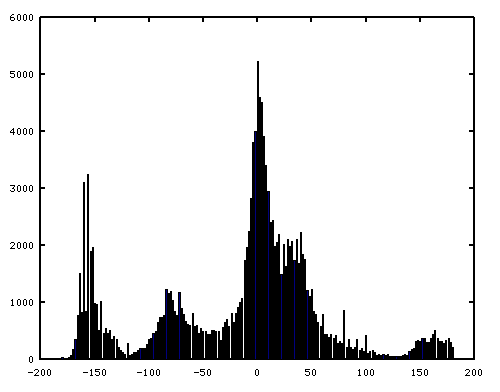
\includegraphics[width=2.5in]{figures/fg-diff-h-distribution.png}
      \caption{Distribution over the difference in hue component for
        object pixels.}
      \label{fig:fg-diff-h-distribution}
    \end{figure}

    The above command will also give you the mean and standard
    deviation of the distribution. You can use them in the next phase.
\end{enumerate}

\subsubsection*{Online Phase}

Given the model estimate $\Theta$, we use the maximum likelihood
approach to classify a pixel as a shadow pixel if
\begin{equation}
  \label{eq:ml}
  P(M_{\text{xy}} \mid A_{xy}=\text{sh} ; \Theta ) >
  P(M_{\text{xy}} \mid A_{xy}=\text{obj} ; \Theta ).
\end{equation}
Otherwise, we classify the pixel as an object pixel. Here we could add
the prior probabilities to the shadow model and the object model in
(\ref{eq:ml}) to obtain a maximum a posteriori classifier. In this
workshop, we can assume equal priors. \\

\noindent To perform the classification:
\begin{enumerate}
  \item Look at the code {\tt shadow\_ml.cc}.
  \item Manually set the parameters in the code for the distributions
    for object pixels and shadow pixels.
  \item Run {\tt make} to compile the code.
  \item Run the program and see the results.
\end{enumerate}

\noindent Also, see the code usage below. \\

\noindent {\tt
Usage: shadow\_ml <video> \\
Option: \\
-T <threshold for background subtraction> \\
-d <delay> \\
}

\noindent If you are interested in the maximum likelihood approach,
you can find our published work~[1] in the reference section. \\

\noindent OK, now we learn how to apply some simple techniques to
detect shadows. Hope you can apply and extend these techniques to
other problems or datasets. :-)

\subsection*{References}

\begin{itemize}
  \item[1] Ouivirach, K., \& Dailey, M.\ N.\ (2010) Clustering human
    behaviors with dynamic time warping and hidden Markov models for a
    video surveillance system. In \textit{ECTI-CON}, (pp.\ 884--888).
\end{itemize}

\end{document}






%\begin{enumerate}
%  \item Create a ROS workspace: \\\\ 
%    \texttt{\$ mkdir
%      {\raise.17ex\hbox{$\scriptstyle\mathtt{\sim}$}}/ros\_workspace}
%  \item It is convenient to set up the ROS workspace automatically
%    every time we open a new terminal. Run the following commands:
%  \begin{enumerate}
%    \item {\tt \$ echo "export
%      ROS\_PACKAGE\_PATH={\raise.17ex\hbox{$\scriptstyle\mathtt{\sim}$}}/ros\_workspace:\$ROS\_PACKAGE\_PATH"
%      >> {\raise.17ex\hbox{$\scriptstyle\mathtt{\sim}$}}/.bashrc}
%    \item {\tt \$ echo "export
%      ROS\_WORKSPACE={\raise.17ex\hbox{$\scriptstyle\mathtt{\sim}$}}/ros\_workspace"
%      >> {\raise.17ex\hbox{$\scriptstyle\mathtt{\sim}$}}/.bashrc}
%    \item {\tt \$
%      . {\raise.17ex\hbox{$\scriptstyle\mathtt{\sim}$}}/.bashrc}
%  \end{enumerate}
%  \item Just to confirm you have done it correctly. Run this command:
%    {\tt echo \$ROS\_PACKAGE\_PATH}, and you should see something
%    similar to: \\\\ 
%    {\tt
%      /home/YOUR\_USER\_NAME/ros\_workspace:/opt/ros/fuerte/share:/opt/ros/fuerte/stacks} \\\\
%    If you are using the different version of ROS, please change the
%    environment accordingly.
%  \item Now if you run: {\tt roscd}, you will go to your workspace
%    directly.
%\end{enumerate}

%\subsection*{Understand ROS with Turtle}

%In this section, a turtle will help you to understand how ROS
%messaging mechanism works.

%\begin{enumerate}
%  \item We get started with building a ROS package {\tt
%    turtlesim}. First we need to install \textit{system dependencies}
%    required for {\tt turtlesim}: \\\\ 
%    {\tt \$ rosdep install turtlesim} \\\\
%    If you see an error saying that {\tt rosdep} has
%    not been initialized. To fix this, run: \\\\ 
%    {\tt \$ sudo rosdep init} \\ {\tt \$ rosdep update}
%  \item Then to build the package, run: \\\\ 
%    {\tt \$ rosmake turtlesim}
%  \item In order for ROS nodes to communicate, you \textbf{must} keep
%    the ROS server running. Open a new terminal and run: \\\\ 
%    {\tt \$ roscore} \\\\ 
%    By default, the server will be run on your local machine. If you
%    want to run nodes across multiple machines, please see
%    \url{http://www.ros.org/wiki/ROS/NetworkSetup} for more
%    information. To see the information about the ROS nodes that are
%    currently running, run: \\\\ 
%    {\tt \$ rosnode list} \\\\ 
%    You will see a node {\tt rosout} that is always running as it
%    collects and logs nodes' debugging output. You may use the
%    following command to see the information about a specific running
%    node: \\\\ 
%    {\tt \$ rosnode info <node-name>}
%  \item Let's summon a turtle. Open a new terminal and run: \\\\ 
%    {\tt \$ rosrun turtlesim turtlesim\_node} \\\\ 
%    This means that you are running the executable {\tt
%      turtlesim\_node} in the package {\tt turtlesim}. OK, by now you
%    should have your little turtle!  Check again (in a new terminal)
%    what nodes are running: \\\\ 
%    {\tt \$ rosnode list} \\\\ 
%    You can ping your turtle to see if it is still alive by this
%    command: \\\\ 
%    {\tt \$ rosnode ping turtlesim} \\\\ 
%    If you want to stop the node, just press {\tt Ctrl-C}.
%  \item Let's control your turtle around. Run an another new node in a
%    new terminal to enable your keyboard to control: \\\\ 
%    {\tt \$ rosrun turtlesim turtle\_teleop\_key} \\\\ 
%    Congratulations!  You can control your little turtle now. :-)
%  \item To understand how messaging mechanism works, run the command
%    below in a new terminal: \\\\
%    {\tt \$ rxgraph} \\\\ 
%    You should see a graph similar to Figure \ref{fig:rxgraph}. In
%    this figure, you can see the ROS nodes and topics. The {\tt
%      turtlesim} and the {\tt teleop\_turtle} nodes are communicating
%    on the topic named \\ {\tt /turtle1/command\_velocity}.

%    \begin{figure}[t]
%      \begin{center}
%        \includegraphics[width=0.8\linewidth]{figures/rxgraph.png}
%      \end{center}
%      \caption{Dynamic graph created by {\tt rxgraph}.}
%      \label{fig:rxgraph}
%    \end{figure}
    
%  \item To see the data published on this topic, run: \\\\ 
%    {\tt \$ rostopic echo /turtle1/command\_velocity} \\\\ 
%    If you check the graph created by {\tt rxgraph} again, you will
%    see a new node has subscribed to the {\tt
%      /turtle1/command\_velocity} topic.
%\end{enumerate}

%\subsection*{Write a Simple ROS Application}

%Say good bye to your turtle. In this section, we will write our own
%application, ``Hello ROS World,'' to get an idea how to write a
%program with ROS in Python! Therefore, you should have Python
%installed on your machine. If not, run: {\tt sudo apt-get install
%  python}.

%\begin{enumerate}
%  \item Let's do it in our workspace so that ROS can find our new
%    package. Simply do: \\\\ 
%    {\tt \$ roscd}
%  \item Create our package: \\\\ 
%    {\tt \$ roscreate-pkg beginner\_tutorials std\_msgs rospy roscpp}
%    \\\\
%    This means that our package {\tt beginner\_tutorials} will depend
%    on {\tt std\_msgs}, {\tt rospy}, and {\tt roscpp}. {\tt std\_msgs}
%    contains common message types, {\tt rospy} is the client library
%    that allows Python to communicate through ROS, and {\tt roscpp} is
%    the client library for C++.
%  \item Make sure ROS can find your package. Run: \\\\ 
%    {\tt \$ rospack find beginner\_tutorials} \\\\ 
%    You should see the output like this: {\tt
%      YOUR\_PACKAGE\_PATH/beginner\_tutorials}.
%  \item To build our package, run: \\\\ 
%    {\tt \$ rosmake beginner\_tutorials}
%  \item Change directory to  our package: \\\\ 
%    {\tt \$ roscd beginner\_tutorials}
%  \item Create a file {\tt talker.py} under {\tt /src}.
%    \begin{enumerate}
%      \item Every node will have this declaration at the top.
%\begin{verbatim}
%#!/usr/bin/env python
%import roslib; roslib.load_manifest('beginner_tutorials')
%\end{verbatim}
%        This tells {\tt roslib} to read in the {\tt manifest.xml} file
%        and add all the dependencies listed there to the {\tt
%          PYTHONPATH}. {\tt roslib.load\_manifest()} also enables us
%        to find both {\tt rospy} and {\tt std\_msgs}, which are
%        declared as dependencies in the {\tt manifest.xml}.
%      \item We can import other libraries as follows.
%\begin{verbatim}
%import rospy
%from std_msgs.msg import String
%\end{verbatim}
%      \item We then define the talker's interface to the rest of ROS
%        as follows.
%\begin{verbatim}
%def talker():
%    pub = rospy.Publisher('chatter', String)
%    rospy.init_node('talker')
%\end{verbatim}
%        We declare that our node will publish to the {\tt chatter}
%        topic using the message type {\tt String}, and we also tell
%        {\tt rospy} the name of the node.
%      \item We will let it run forever until we press {\tt Ctrl-C} or
%        otherwise. See the code below.
%\begin{verbatim}
%    while not rospy.is_shutdown():
%        # substitute the time to the message
%        str = 'Hello ROS World %s' % rospy.get_time()
%        # loginfo()
%        # gets the message printed to screen
%        # gets it written to the Node's log file
%        # gets it written to rosout
%        rospy.loginfo(str)
%        pub.publish(String(str))
%        rospy.sleep(1.0)
%\end{verbatim}
%        Here the real work is {\tt pub.publish(String(str))} that
%        keeps publishing the message to the {\tt chatter} topic.
%    \item Here is the entire code.
%\begin{verbatim}
%#!/usr/bin/env python
%import roslib; roslib.load_manifest('beginner_tutorials')
%import rospy
%from std_msgs.msg import String

%def talker():
%    pub = rospy.Publisher('chatter', String)
%    rospy.init_node('talker')
%    while not rospy.is_shutdown():
%        str = 'Hello ROS World %s' % rospy.get_time()
%        rospy.loginfo(str)
%        pub.publish(String(str))
%        rospy.sleep(1.0)

%if __name__ == '__main__':
%    talker()
%\end{verbatim}
%    \item We need to make the node executable. Run: \\\\ 
%      {\tt \$ chmod +x src/talker.py}
%  \end{enumerate}
%  \item We also need to write a node to receive the messages. Create a
%    file {\tt listener.py} under {\tt /src}.
%    \begin{enumerate}
%      \item The code will look similar to {\tt talker.py}, except we
%        need to first write a callback function for handling the messages as
%        follows.
%\begin{verbatim}
%def callback(data):
%    rospy.loginfo(rospy.get_name() + 'I heard %s', data.data)
%\end{verbatim}
%      \item We then subscribe to the {\tt chatter} topic as follows.
%\begin{verbatim}
%def listener():
%    rospy.init_node('listener', anonymous=True)
%    rospy.Subscriber('chatter', String, callback)
%    rospy.spin()
%\end{verbatim}
%        When new messages are received, {\tt callback} is invoked with
%        the message as the first argument. The {\tt anonymous=True}
%        flag tells {\tt rospy} to generate a unique name for the node
%        so that you can have multiple {\tt listener.py} nodes run
%        easily. In the last line of this function, {\tt rospy.spin()}
%        simply keeps the node from exiting until the node has been
%        shutdown.
%      \item Here is the entire code.
%\begin{verbatim}
%#!/usr/bin/env python
%import roslib; roslib.load_manifest('beginner_tutorials')
%import rospy
%from std_msgs.msg import String
%
%def callback(data):
%    rospy.loginfo(rospy.get_name() + "I heard %s", data.data)
 
%def listener():
%    rospy.init_node('listener', anonymous=True)
%    rospy.Subscriber("chatter", String, callback)
%    rospy.spin()
% 
%if __name__ == '__main__':
%    listener()
%\end{verbatim}
%      \item Again, we need to make the node executable. Run: \\\\ 
%        {\tt \$ chmod +x src/listener.py}
%    \end{enumerate}
%  \item Even you write a program in Python, you still have to build it
%    to make sure that the ROS creates the auto-generated Python code
%    for messages and services. Run: \\\\ 
%    {\tt \$ rosmake beginner\_tutorials}
%  \item After that, open a new terminal and then start the ROS server:
%    \\\\
%    {\tt \$ roscore} \\\\ 
%    Run the Talker in a new terminal: \\\\ 
%    {\tt \$ rosrun beginner\_tutorials talker.py} \\\\ 
%    Also, run the Listener in a new terminal: \\\\ 
%    {\tt \$ rosrun beginner\_tutorials listener.py} \\\\ 
%    Your task now is to try to understand the results.
%  \item After we understand how it works, please exit all of the
%    current running program, except the ROS server. We will try
%    another command {\tt roslaunch} to start nodes. In the real
%    projects, we usually execute this command to start all nodes we
%    want rather than start one of them one by one. Your life will be
%    easier.
%  \item Let's create a subfolder {\tt launch} under our package so
%    that {\tt roslaunch} can automatically find our launch file.
%  \item Create a simple launch file {\tt hello.launch} and paste the
%    following:
%\begin{verbatim}
%<launch>
%    <node name="listener" pkg="beginner_tutorials" type="listener.py" />
%    <node name="talkerPy" pkg="beginner_tutorials" type="talker.py" />
%</launch>
%\end{verbatim}
%    This means we will create two nodes: {\tt listener} and {\tt
%      talkerPy} by running {\tt listener.py} and {\tt talker.py},
%    respectively. Please see \url{http://ros.org/wiki/roslaunch/XML}
%    for more information about the XML format used for {\tt
%      roslaunch}. \\\\
%    Now we start the ROS server and then run the following command in
%    a new terminal: \\\\ 
%    {\tt \$ roslaunch beginner\_tutorial hello.launch}
%  \item Run the following command the see which nodes are currently
%    running: \\\\ 
%    {\tt \$ rosnode list} \\\\ 
%    The see the dynamic graph, run: \\\\ 
%    {\tt \$ rxgraph} \\\\ 
%    To see the messages being passed, run: \\\\ 
%    {\tt \$ rostopic echo chatter} \\
%\end{enumerate}

%\noindent Congratulations again! We have studied the frequently used
%command-line tools, we understand the communication between nodes, and
%we can implement a simple publisher and subscriber with ROS. For more
%advanced information, I would encourage you to see the references
%provided at the end.

%\subsubsection*{[Optional] What if Another Talker is Implemented in C++?}

%In this section, you may download a modified version of Talker from
%\url{http://se.cs.ait.ac.th/~kan/cloud-robotics/talker.cpp} or follow
%this instructions:
%\\ \url{http://www.ros.org/wiki/ROS/Tutorials/WritingPublisherSubscriber(c++)}
%\\

%\noindent Let's follow these steps below.
%\begin{enumerate}
%  \item Put {\tt talker.cpp} under {\tt /src}.
%  \item Change directory to your package: \\\\ 
%    {\tt \$ roscd beginner\_tutorials}
%  \item Before we build the package, we need to add the following line
%    at the bottom of {\tt CMakeLists.txt}. \\\\ 
%    {\tt rosbuild\_add\_executable(talker src/talker.cpp)}
%  \item Run {\tt make} then you can see that the executable file {\tt
%    talker} is created and goes into the {\tt /bin} directory by
%    default.
%  \item Finally, run the ROS server, Listener, Talker (Python), and
%    Talker (C++) in the \textit{different} terminals using {\tt
%      rosrun}. See the results. You are expected to see an error at
%    Talker (Python). Why?  :-)
%  \item Fix it. Good luck! (Hint: {\tt roslaunch})
%\end{enumerate}



